%
% ritzloesung.tex
%
% (c) 2024 Prof Dr Andreas Müller
%
\begin{figure}
\centering
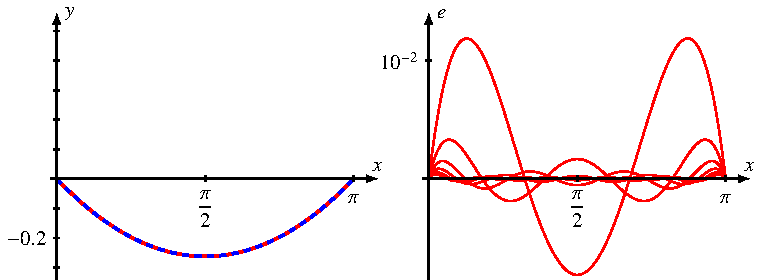
\includegraphics{chapters/070-direkt/images/ritzloesung.pdf}
\caption{Lösung des Refraktionsproblems mit dem Ritzverfahren.
Die numerische Lösung mit dem Ritz-Verfahren (rot) ist visuell nicht von
der Lösung der Euler-Lagrange-Differentialgleichung zu unterscheiden.
Der Unterschied $y_n(x)-y_\infty(x)$ ist rechts hundertfach überhöht
dargestellt.
Mit nur sechs Termen findet das Ritz-Verfahren eine Lösung mit einem
Fehler $<10^{-3}$.
\label{buch:direkt:ritz:fig:ritzloesung}}
\end{figure}
